
\de{ĐỀ THI HỌC KỲ I NĂM HỌC 2022-2023}{Trường THPT  Quế Sơn - Quảng Nam}
\begin{center}
	\textbf{PHẦN 1 - TRẮC NGHIỆM}
\end{center}
\Opensolutionfile{ans}[ans/ans]

\begin{ex}%[0D1Y1-1]%[Dự án đề kiểm tra HK1 NH22-23 - Lê Hùng Thắng]%[THPT Quế Sơn - Quảng Nam]%Câu 1
Trong các câu sau, câu nào không phải là mệnh đề?
\choice
{\True Hãy làm bài kiểm tra thật nghiêm túc!}
{Hà Nội là thủ đô của Việt Nam}
{$7$ là số nguyên tố}
{$8+2=11$}
\loigiai{
Câu không phải mệnh đề là ``Hãy làm bài kiểm tra thật nghiêm túc!''.\\
Đây là câu mệnh lệnh.
}%<MyLT1>
\end{ex}

\begin{ex}%[0D1Y2-3]%[Dự án đề kiểm tra HK1 NH22-23 - Lê Hùng Thắng]%[THPT Quế Sơn - Quảng Nam]%Câu 2
Cho tập hợp $M=\{x\in\mathbb{R}\mid x^2+3x-4=0\}$. Tập $M$ được viết lại là
\choice
{$M=\{-1;4\}$}
{\True $M=\{-4;1\}$}
{$M=(-1;4)$}
{$M=(-4;1)$}
\loigiai{
	Ta có $x^2+3x-4=0 \Leftrightarrow \left[\begin{aligned}
	&x=1\\	&x=-4.\\
	\end{aligned}\right.$\\
Vậy $M=\{-4;1\}$.
}%<MyLT1>
\end{ex}

\begin{ex}%[0D1B3-4]%[Dự án đề kiểm tra HK1 NH22-23 - Lê Hùng Thắng]%[THPT Quế Sơn - Quảng Nam]%Câu 3
Cho $2$ tập hợp $M=(-\infty ;-1]$, $N=(-2;4]$. Mệnh đề nào sau đây \textbf{đúng}?
\choice
{$M\cap N=(-\infty; 4]$}
{$M\cap N=(-\infty; 4)$}
{$M\cap N=[-2; -1)$}
{\True $M\cap N=(-2; -1]$}
\loigiai{
	Ta có $M\cap N=(-\infty ;-1]\cap (-2;4]=(-2; -1]$.
}%<MyLT1>
\end{ex}

\begin{ex}%[0D2Y1-2]%[Dự án đề kiểm tra HK1 NH22-23 - Lê Hùng Thắng]%[THPT Quế Sơn - Quảng Nam]%Câu 4
Trong mặt phẳng tọa độ, điểm nào sau đây thuộc miền nghiệm của bất phương trình bậc nhất hai ẩn $x+2y \ge 3$?
\choice
{$A(-2; -1)$}
{\True $B(-1; 2)$}
{$C(1; -2)$}
{$D(2; 0)$}
\loigiai{
	Thay tọa độ $B(-1; 2)$ vào bất phương trình, ta có $-1+2\cdot 2 \ge 3$ là mệnh đề đúng.\\
	Vậy $B(-1; 2)$ thuộc miền nghiệm của bất phương trình bậc nhất hai ẩn đã cho.
}%<MyLT1>
\end{ex}

\begin{ex}%[0D2B2-2]%[Dự án đề kiểm tra HK1 NH22-23 - Lê Hùng Thắng]%[THPT Quế Sơn - Quảng Nam]%Câu 5
Cho hệ bất phương trình bậc nhất $2$ ẩn $\left\{\begin{aligned}
& x-y<0\\ & x+2y\ge 0\\ \end{aligned}\right.$. Cặp số nào sau đây \textbf{không} phải là nghiệm của hệ đã cho?
\choice
{$(0;1)$}
{$(1;2)$}
{$(-2;1)$}
{\True $(0;-3)$}
\loigiai{
	Thay $(x;y)=(0;-3)$ vào hệ bất phương trình ta thấy không thỏa.\\
	Vậy $(0;-3)$ không phải là nghiệm của hệ bất phương trình đã cho.
}%<MyLT1>
\end{ex}

\begin{ex}%[0H1Y1-3]%[Dự án đề kiểm tra HK1 NH22-23 - Lê Hùng Thắng]%[THPT Quế Sơn - Quảng Nam]%Câu 6
Cho $\alpha$ và $\beta$ là hai góc khác nhau và bù nhau. Trong các đẳng thức sau đây, đẳng thức nào sai?
\choice
{$\sin\alpha=\sin\beta$}
{$\cos\alpha=-\cos\beta$}
{$\tan\alpha=-\tan\beta$}
{\True $\cot\alpha=\cot\beta$}
\loigiai{
Với $\alpha$ và $\beta$ là hai góc khác nhau và bù nhau ta có $\cot\alpha=-\cot\beta$.\\
Vậy đẳng thức $\cot\alpha=\cot\beta$ là đẳng thức sai.
}%<MyLT1>
\end{ex}

\begin{ex}%[0H1Y2-2]%[Dự án đề kiểm tra HK1 NH22-23 - Lê Hùng Thắng]%[THPT Quế Sơn - Quảng Nam]%Câu 7
Trong tam giác $ABC$, gọi $p, R, r, S$ lần lượt là nửa chu vi, bán kính đường tròn ngoại tiếp, bán kính đường tròn nội tiếp và diện tích của tam giác $ABC$. Khẳng định nào sau đây đúng?
\choice
{$S=2ab\sin C$}
{$S=\dfrac{abc}{4r}$}
{\True $\dfrac{b}{\sin B}=2R$}
{$S=p\cdot R$}
\loigiai{
 Ta có $\dfrac{b}{\sin B}=2R$ là đẳng thức đúng.\\
 Các đẳng thức còn lại đều sai.
}%<MyLT1>
\end{ex}

\begin{ex}%[0H2B1-2]%[Dự án đề kiểm tra HK1 NH22-23 - Lê Hùng Thắng]%[THPT Quế Sơn - Quảng Nam]%Câu 8
Trên đoạn thẳng $MN$, lấy điểm $P$ nằm giữa 2 điểm $M,N$. Phát biểu nào sau đây đúng?
\choice
{Hai véc-tơ $\overrightarrow{MN}$ và $\overrightarrow{MP}$ ngược hướng}
{Hai véc-tơ $\overrightarrow{PN}$ và $\overrightarrow{MP}$ ngược hướng}
{\True Hai véc-tơ $\overrightarrow{NM}$ và $\overrightarrow{MP}$ cùng phương}
{Hai véc-tơ $\overrightarrow{PM}$ và $\overrightarrow{PN}$ cùng hướng}
\loigiai{
	\begin{center}
	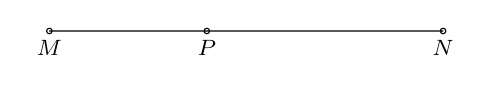
\begin{tikzpicture}[scale=1,>=stealth, font=\footnotesize, line join=round, line cap=round]
	\draw (0,0) circle (1pt) node [below] {$M$}--
	(2,0) circle (1pt) node [below] {$P$}--
	(5,0) circle (1pt) node [below] {$N$};
	\end{tikzpicture}
	\end{center}
Do ba điểm $M,N,P$ thẳng hàng nên phát biểu ``Hai véc-tơ $\overrightarrow{NM}$ và $\overrightarrow{MP}$ cùng phương'' là đúng.\\
Các phát biểu còn lại đều sai.
}%<MyLT1>
\end{ex}

\begin{ex}%[0H2Y2-3]%[Dự án đề kiểm tra HK1 NH22-23 - Lê Hùng Thắng]%[THPT Quế Sơn - Quảng Nam]%Câu 9
Cho $3$ điểm $A, B, C$ tùy ý. Đẳng thức nào sau đây \textbf{sai}?
\choice
{$\overrightarrow{CA}+\overrightarrow{AB}=\overrightarrow{CB}$}
{$\overrightarrow{AB}-\overrightarrow{AC}=\overrightarrow{CB}$}
{$\overrightarrow{BA}+\overrightarrow{AC}=\overrightarrow{BC}$}
{\True $\overrightarrow{CA}-\overrightarrow{CB}=\overrightarrow{AB}$}
\loigiai{ Ta có $\overrightarrow{CA}-\overrightarrow{CB}=\overrightarrow{BA}$.\\
	Vậy đẳng thức $\overrightarrow{CA}-\overrightarrow{CB}=\overrightarrow{AB}$ là đẳng thức sai.
}%<MyLT1>
\end{ex}

\begin{ex}%[0H2B3-2]%[Dự án đề kiểm tra HK1 NH22-23 - Lê Hùng Thắng]%[THPT Quế Sơn - Quảng Nam]%Câu 10
Cho $\triangle ABC$ có $G$ là trọng tâm, $I$ là trung điểm $BC$. Đẳng thức nào sau đây đúng?
\choice
{$\overrightarrow{GA}=2\overrightarrow{GI}$}
{$\overrightarrow{IG}=-\dfrac{1}{3}\overrightarrow{IA}$}
{\True $\overrightarrow{GB}+\overrightarrow{GC}=2\overrightarrow{GI}$}
{$\overrightarrow{GB}+\overrightarrow{GC}=\overrightarrow{GA}$}
\loigiai{
\immini{Dựa vào hình vẽ ta có đẳng thức $\overrightarrow{GB}+\overrightarrow{GC}=2\overrightarrow{GI}$ là đẳng thức đúng.\\
	Các đẳng thức còn lại đều sai.
}
{	\begin{tikzpicture}[scale=1,>=stealth, font=\footnotesize, line join=round, line cap=round]
	\path (1,3) coordinate (A)
	 (0,0) coordinate (B)
 (5,0) coordinate (C)
 ($(B)!0.5!(C)$) coordinate (I)
 ($(A)!2/3!(I)$) coordinate (G);
	\draw (A)--(B)--(C)--(A)--(I);
	\foreach \d/\g in {A/1600,B/180,C/0,I/-90,G/20} \fill (\d) circle (1pt) ++(\g:3mm) node {$\d$};
	\end{tikzpicture}
}
}%<MyLT1>
\end{ex}

\begin{ex}%[0H2B3-1]%[Dự án đề kiểm tra HK1 NH22-23 - Lê Hùng Thắng]%[THPT Quế Sơn - Quảng Nam]%Câu 11
Trên đoạn thẳng $AC$, cho điểm $B$ nằm giữa hai điểm $A$ và $C$, với $AB=2a$, $AC=8a$. Đẳng thức nào dưới đây đúng?
\choice
{\True $\overrightarrow{BC}=-3\overrightarrow{BA}$}
{$\overrightarrow{AB}=4\overrightarrow{CA}$}
{$\overrightarrow{BC}=4\overrightarrow{AB}$}
{$\overrightarrow{AC}=-4\overrightarrow{AB}$}
\loigiai{
	\begin{center}
	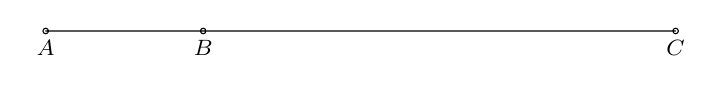
\begin{tikzpicture}[scale=1,>=stealth, font=\footnotesize, line join=round, line cap=round]
	\draw (0,0) circle (1pt) node [below] {$A$}--
	(2,0) circle (1pt) node [below] {$B$}--
	(8,0) circle (1pt) node [below] {$C$};
	\end{tikzpicture}
	\end{center}
Dựa vào hình vẽ ta có đẳng thức $\overrightarrow{BC}=-3\overrightarrow{BA}$ là đẳng thức đúng.\\
Các đẳng thức còn lại đều sai.
}%<MyLT1>
\end{ex}

\begin{ex}%[0H3Y1-3]%[Dự án đề kiểm tra HK1 NH22-23 - Lê Hùng Thắng]%[THPT Quế Sơn - Quảng Nam]%Câu 12
Trong mặt phẳng $Oxy$, cho $\overrightarrow{a}=(1;2),\overrightarrow{b}=(3;8)$. Véc-tơ $\overrightarrow{c}=2\overrightarrow{a}-\overrightarrow{b}$ có tọa độ là
\choice
{\True $\overrightarrow{c}=(-1;-4)$}
{$\overrightarrow{c}=(5;12)$}
{$\overrightarrow{c}=(2;5)$}
{$\overrightarrow{c}=(2;6)$}
\loigiai{
	Ta có $\overrightarrow{c}=2\overrightarrow{a}-\overrightarrow{b}
	=(2\cdot 1-3;2\cdot 2-8)=(-1;-4)$.	
}%<MyLT1>
\end{ex}

\begin{ex}%[0H3Y1-3]%[Dự án đề kiểm tra HK1 NH22-23 - Lê Hùng Thắng]%[THPT Quế Sơn - Quảng Nam]%Câu 13
Trong mặt phẳng $Oxy$, cho $2$ điểm $M(-2;-3)$, $N(4;5)$. Tọa độ véc-tơ $\overrightarrow{MN}$ là
\choice
{$\overrightarrow{MN}=(1;1)$}
{$\overrightarrow{MN}=(2;2)$}
{\True $\overrightarrow{MN}=(6;8)$}
{$\overrightarrow{MN}=(-6;-8)$}
\loigiai{
Ta có $\overrightarrow{MN}=(4-(-2);5-(-3))=(6;8)$.
}%<MyLT1>
\end{ex}

\begin{ex}%[0H3Y1-3]%[Dự án đề kiểm tra HK1 NH22-23 - Lê Hùng Thắng]%[THPT Quế Sơn - Quảng Nam]%Câu 14
Trong mặt phẳng $Oxy$, cho $A(2;-3)$, $B(2;7)$. Tọa độ trung điểm $I$ của đoạn thẳng $AB$ là
\choice
{$I(4;4)$}
{\True $I(2;2)$}
{$I(0;-10)$}
{$I(0;10)$}
\loigiai{
 $I$ là trung điểm của $AB$ nên ta có $I(2;2)$.
}%<MyLT1>
\end{ex}

\begin{ex}%[0H2B4-1]%[Dự án đề kiểm tra HK1 NH22-23 - Lê Hùng Thắng]%[THPT Quế Sơn - Quảng Nam]%Câu 15
Cho tam giác $ABC$ vuông tại $A$ có $\widehat{B}=60^\circ$. Số đo góc giữa hai véc-tơ $\overrightarrow{CA}$ và $\overrightarrow{CB}$ là
\choice
{$\left(\overrightarrow{CA},\overrightarrow{CB}\right)=150^\circ$}
{$\left(\overrightarrow{CA},\overrightarrow{CB}\right)=60^\circ$}
{$\left(\overrightarrow{CA},\overrightarrow{CB}\right)=120^\circ$}
{\True $\left(\overrightarrow{CA},\overrightarrow{CB}\right)=30^\circ$}
\loigiai{
\immini{
Ta có $\left(\overrightarrow{CA},\overrightarrow{CB}\right)=\widehat{ACB}=30^\circ$.
}
{	\begin{tikzpicture}[scale=1,>=stealth, font=\footnotesize, line join=round, line cap=round]
	\path (0,0) coordinate (A)
	(0,3) coordinate (B)
	(5,0) coordinate (C);
	\draw (A)--(B)--(C)--(A);
	\foreach \d/\g in {A/1600,B/180,C/0} \fill (\d) circle (1pt) ++(\g:3mm) node {$\d$};
	\tkzMarkRightAngles[size=0.17](C,A,B)
	\tkzMarkAngles[size=0.4cm,arc=l,mark=](A,B,C)
	\tkzLabelAngles[pos=0.7,rotate=0](A,B,C){$60^\circ$}
	\end{tikzpicture}
}
}%<MyLT1>
\end{ex}


\Closesolutionfile{ans}
%\begin{center}
%	\textbf{ĐÁP ÁN}
%	\inputansbox{10}{ans/ans}	
%\end{center}
\begin{center}
	\textbf{PHẦN 2 - TỰ LUẬN}
\end{center}


\begin{bt}%[0H1B3-2]%[Dự án đề kiểm tra HKII NH22-23- Nguyễn Ngọc Nguyên]%[THPT Quế Sơn - Quảng Nam]
Hai chiếc tàu thủy cùng xuất phát từ một vị trí $A$, đi thẳng theo hai hướng tạo với nhau một góc $120^{\circ}$. Tàu thứ nhất chạy với vận tốc $50\mathrm{km/h}$, tàu thứ hai chạy với vận tốc $40\mathrm{km/h}$. Hỏi sau $1$ giờ hai tàu cách nhau bao nhiêu $\mathrm{km}$?	
\loigiai{
\begin{center}
	\begin{tikzpicture}[scale=0.85,>=stealth, font=\footnotesize, line join=round, line cap=round]
		\def\r{3};
		\def\gocb{0};
		\def\gocc{120};
		\path 
		(0,0) coordinate (A)
		(\gocb:\r) coordinate (B)
		(\gocc:\r) coordinate (C)
		;
		\draw[->] (A) node[below] {$A$}--(B) node[right] {$B$};
		\draw[->] (A)--(C) node[above] {$C$}; 
		\draw (B)--(C);
		\foreach \x/\y/\z in {B/A/C} \draw pic[draw=black, angle radius=0.45cm,"\tiny $120^{\circ}$"]{angle=\x--\y--\z};
	\end{tikzpicture}
\end{center}
Gọi $B$, $C$ lần lượt là vị trí của tàu thứ nhất và tàu thứ hai đến sau $1$ giờ. Khoảng cách giữa $2$ tàu sau một giờ là độ dài $BC$ (hình minh họa).\\
Ta có $AB=c=50$, $AC=b=40$ và $\widehat{BAC}=\widehat{A}=120^{\circ}$.\\
Áp dụng định lý cô-sin trong tam giác $ABC$ ta có
\begin{eqnarray*}
	BC^2=a^2=b^2+c^2-2bc \cdot \cos A = 50^2+40^2 -2 \cdot 50 \cdot 40 \cdot \cos 120^{\circ}=6100.
\end{eqnarray*}
Vậy $BC=10\sqrt{61} \mathrm{km}$.
}
\end{bt}
\begin{bt}%[0H2B1-5]%[Dự án đề kiểm tra HKII NH22-23- Nguyễn Ngọc Nguyên]%[THPT Quế Sơn - Quảng Nam]
	Cho hình vuông $ABCD$ có cạnh bằng $a$. Tính độ dài các véc-tơ $\overrightarrow{AC}-\overrightarrow{AD}$, $\overrightarrow{AB}+\overrightarrow{BC}$ theo $a$.
	\loigiai{
\immini{
Ta có $\left|  \overrightarrow{AC} - \overrightarrow{AD}\right |=\left |\overrightarrow{DC}\right |=DC=a$.\\
Ta có $\left| \overrightarrow{AB} + \overrightarrow{BC}\right |=\left | \overrightarrow{AC} \right |=AC=\sqrt{AB^2+BC^2}=\sqrt{a^2+a^2}=a\sqrt{2}$.
}
{
\begin{tikzpicture}[scale=0.85,>=stealth, font=\footnotesize, line join=round, line cap=round]
	\path 
	(0,0) coordinate (A) 
	(3,0) coordinate (B) 
	(3,3) coordinate (C) 
	(0,3) coordinate (D) 
	;
	\draw (A)--(B)--(C)--(D)--cycle;
	\foreach \t/\g in {A/-90,B/-90,C/90,D/90}{\draw[fill=white] (\t) circle (1pt) node[shift={(\g:8pt)},font=\footnotesize]{$ \t $};
	}
\end{tikzpicture}
}		
	}
\end{bt}

\begin{bt}%[0H2K3-5]%[Dự án đề kiểm tra HKII NH22-23- Nguyễn Ngọc Nguyên]%[THPT Quế Sơn - Quảng Nam]
	Cho tam giác $ABC$ có trung tuyến $AI$. Gọi $M$ là trung điểm của $AI$, $H$ là điểm thuộc cạnh $AC$ sao cho $AH=4HC$. Chứng minh rằng $20\overrightarrow{MH}=11\overrightarrow{AC}-5\overrightarrow{AB}$.
	\loigiai{
\immini{
Ta có
\begin{eqnarray*}
	\overrightarrow{MH}&=&\overrightarrow{AH}-\overrightarrow{AM} = \dfrac{4}{5}\overrightarrow{AC}-\dfrac{1}{2}\overrightarrow{AI} \\
	 &=& \dfrac{4}{5} \overrightarrow{AC} - \dfrac{1}{2} \cdot \dfrac{1}{2} \left(\overrightarrow{AB}+\overrightarrow{AC}\right)=\dfrac{11}{20}\overrightarrow{AC}-\dfrac{1}{4}\overrightarrow{AB}
\end{eqnarray*}
Từ đó suy ra $20\overrightarrow{MH}=11\overrightarrow{AC}-5\overrightarrow{AB}$.
}
{
\begin{tikzpicture}[scale=0.85,>=stealth, font=\footnotesize, line join=round, line cap=round]
	\path 
	(0,0) coordinate (A)
	(-3,-5) coordinate (B)
	(4,-3) coordinate (C)
	($(C)!0.5!(B)$) coordinate (I)
	($(A)!0.5!(I)$) coordinate (M)
	($(A)!0.8!(C)$) coordinate (H)
	;
	\draw (A)--(B)--(C)--cycle;
	\draw (A)--(I) (M)--(H);
	\foreach \t/\g in {A/90,B/-90,C/-90,I/-90,M/180,H/45}{\draw[fill=white] (\t) circle (1pt) node[shift={(\g:8pt)},font=\footnotesize]{$ \t $};
	}
	\foreach \x/\y in {B/I,C/I}{
		\path (\x)--(\y) node[midway,sloped]{\tikz{\draw[thick,teal] (-90:2pt)--(90:2pt);}};
	}
	\foreach \x/\y in {A/M,M/I}{
	\path (\x)--(\y) node[midway,sloped]{\tikz{\draw[shift={(-0.65pt,0)}](-90:2pt)--(90:2pt) [shift={(0.65pt,0)}](-90:2pt)--(90:2pt);}};
}
\end{tikzpicture}
}		
	}
\end{bt}

\begin{bt}%[0H3K2-5]%[Dự án đề kiểm tra HKII NH22-23- Nguyễn Ngọc Nguyên]%[THPT Quế Sơn - Quảng Nam]
	Trong mặt phẳng tọa độ $Oxy$, cho hình bình hành $ABCD$ có $B(1;2)$, $D(3;-1)$.
	\begin{enumerate}
		\item Tìm tọa độ điểm $P$ trên trục $Ox$ sao cho tam giác $BDP$ vuông tại $D$.
		\item Gọi $Q$ là trung điểm của cạnh $BC$, $N$ là giao điểm của $AC$ và $DQ$. Biết $N(2;-1)$, tìm tọa độ các điểm $A$, $C$.
	\end{enumerate}
	\loigiai{
\immini{\begin{enumerate}
	\item Vì $P \in Ox$ nên $P(x;0)$.\\
	Ta có $\overrightarrow{DB}=(-2;3)$; $\overrightarrow{DP}=(x-3;1)$.\\
	Tam giác $BDP$ vuông tại $D$ khi và chỉ khi 
	\begin{eqnarray*}
		&&\overrightarrow{DB} \perp \overrightarrow{DP} \Leftrightarrow \overrightarrow{DB} \cdot \overrightarrow{DP}=0 \\
		&\Leftrightarrow& -2(x-3)+3\cdot 1 =0 \Leftrightarrow x=\dfrac{9}{2}.
	\end{eqnarray*}
	Vậy $P\left( \dfrac{9}{2};0\right)$.
	\item Gọi $I$ là tâm của hình bình hành $ABCD$, xét tam giác $BCD$ có $CI$ và $DQ$ là hai đường trung tuyến nên $N$ là trọng tâm. Do đó
	\begin{eqnarray*}
		\heva{&2=\dfrac{1+x_C+3}{3} \\ & -1=\dfrac{2+y_C-1}{3}} \Leftrightarrow \heva{&x_C=2 \\ &y_C=-4.} \Rightarrow C(2;-4).
	\end{eqnarray*}
Ta có $$\overrightarrow{CA}=3\overrightarrow{CN} \Leftrightarrow \heva{&x_A - x_C =3 \left( x_N-x_C \right) \\ &y_A - y_C =3 \left( y_N-y_C \right) } \Leftrightarrow \heva{&x_A-2=3(2-2) \\ & y_A+4=3(-1+4)} \Leftrightarrow \heva{&x_A=2 \\ &y_A=5} \Rightarrow A(2;5).$$
\end{enumerate}
}
{
\begin{tikzpicture}[scale=0.85,>=stealth, font=\footnotesize, line join=round, line cap=round]
	\path 
	(0,0) coordinate (A)
	(4,0) coordinate (B)
	(5,3) coordinate (C)
	($(A)+(C)-(B)$) coordinate (D)
	($(A)!0.5!(C)$) coordinate (I)
	($(I)!1/3!(C)$) coordinate (N)
	($(B)!0.5!(C)$) coordinate (Q)
	;
	\draw (A)--(B)--(C)--(D)--(A)--(C) (B)--(D) (D)--(Q);
	\foreach \t/\g in {A/-90,B/-90,C/90,D/90,I/90,Q/0,N/-90}{\draw[fill=white] (\t) circle (1pt) node[shift={(\g:8pt)},font=\footnotesize]{$ \t $};
	}
	\foreach \x/\y in {B/Q,C/Q}{
	\path (\x)--(\y) node[midway,sloped]{\tikz{\draw[thick,teal] (-90:2pt)--(90:2pt);}};
}
\end{tikzpicture}
}		
	}
\end{bt}